\begin{figure}[t]
  \centering
  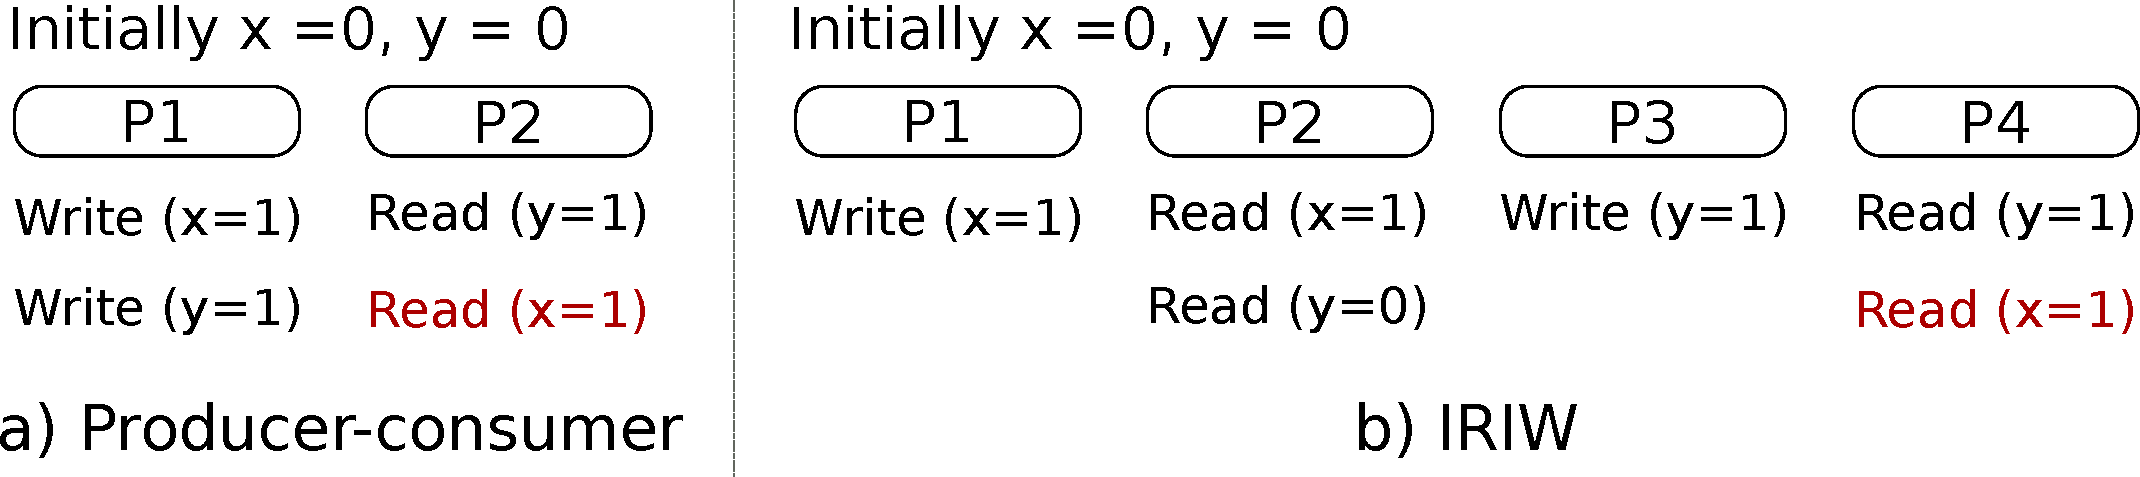
\includegraphics[width=0.48\textwidth]{1_figures/intro-example.pdf}
  \caption{a) The producer-consumer synchronization pattern mandates that if P2 reads P1's write to $y$, then it must also read P1's write to $x$. b) The independent-reads independent-writes (IRIW) pattern mandates that if P2 sees P1's writes but not P3's and P4 sees P3's write, then P4 must see P1's write. }
  \label{fig:intro-ex}
\end{figure}